\documentclass{beamer}

\graphicspath{{img/}}

\usepackage{appendixnumberbeamer}

\usepackage{datetime}
\newdate{defensedate}{21}{01}{2018}

\usepackage{minted}

\usetheme[sectionpage=progressbar,subsectionpage=progressbar,numbering=fraction,
          progressbar=foot]{metropolis}

\usepackage{amssymb}
\usepackage{dirtytalk}
\usepackage{mdframed}
\usepackage{xcolor}

% \usepackage[inline]{enumitem}

\title{Exact Analysis of the Cache Behavior of Nested Loops~\cite{chatterjee2001exact}}

\date{\displaydate{defensedate}}
\author{%
  Simon Bihel\hfill\url{simon.bihel@ens-rennes.fr} \\
}
\institute{%
  University of Rennes I \\
  \'Ecole Normale Sup\'erieure de Rennes
}

\begin{document}

\maketitle

\begin{frame}{Introduction}
  \begin{itemize}
    \item Predict cache behavior (i.e.\ count misses) for performance evaluation
    \item Exact prediction can be done with simulation but it is expensive
    \item Models permit simpler computations
  \end{itemize}
\end{frame}

\begin{frame}{Table of contents}
  \setbeamertemplate{section in toc}[sections numbered]
  \tableofcontents[hideallsubsections]
\end{frame}


\section{Context}

\begin{frame}{Memory Hierarchies}
  \begin{itemize}
    \item 2 levels, one access at a time, no distinction between reads and writes
    \item Least Recently Used replacement policy
  \end{itemize}

  \pause{}

  2 kinds of cache misses
  \begin{description}
    \item[Interior misses] Independent to the initial cache state.
    \item[Boundary misses] Depend on the initial cache state.
  \end{description}
\end{frame}

\begin{frame}{Polyhedral Model}
  \begin{center}
    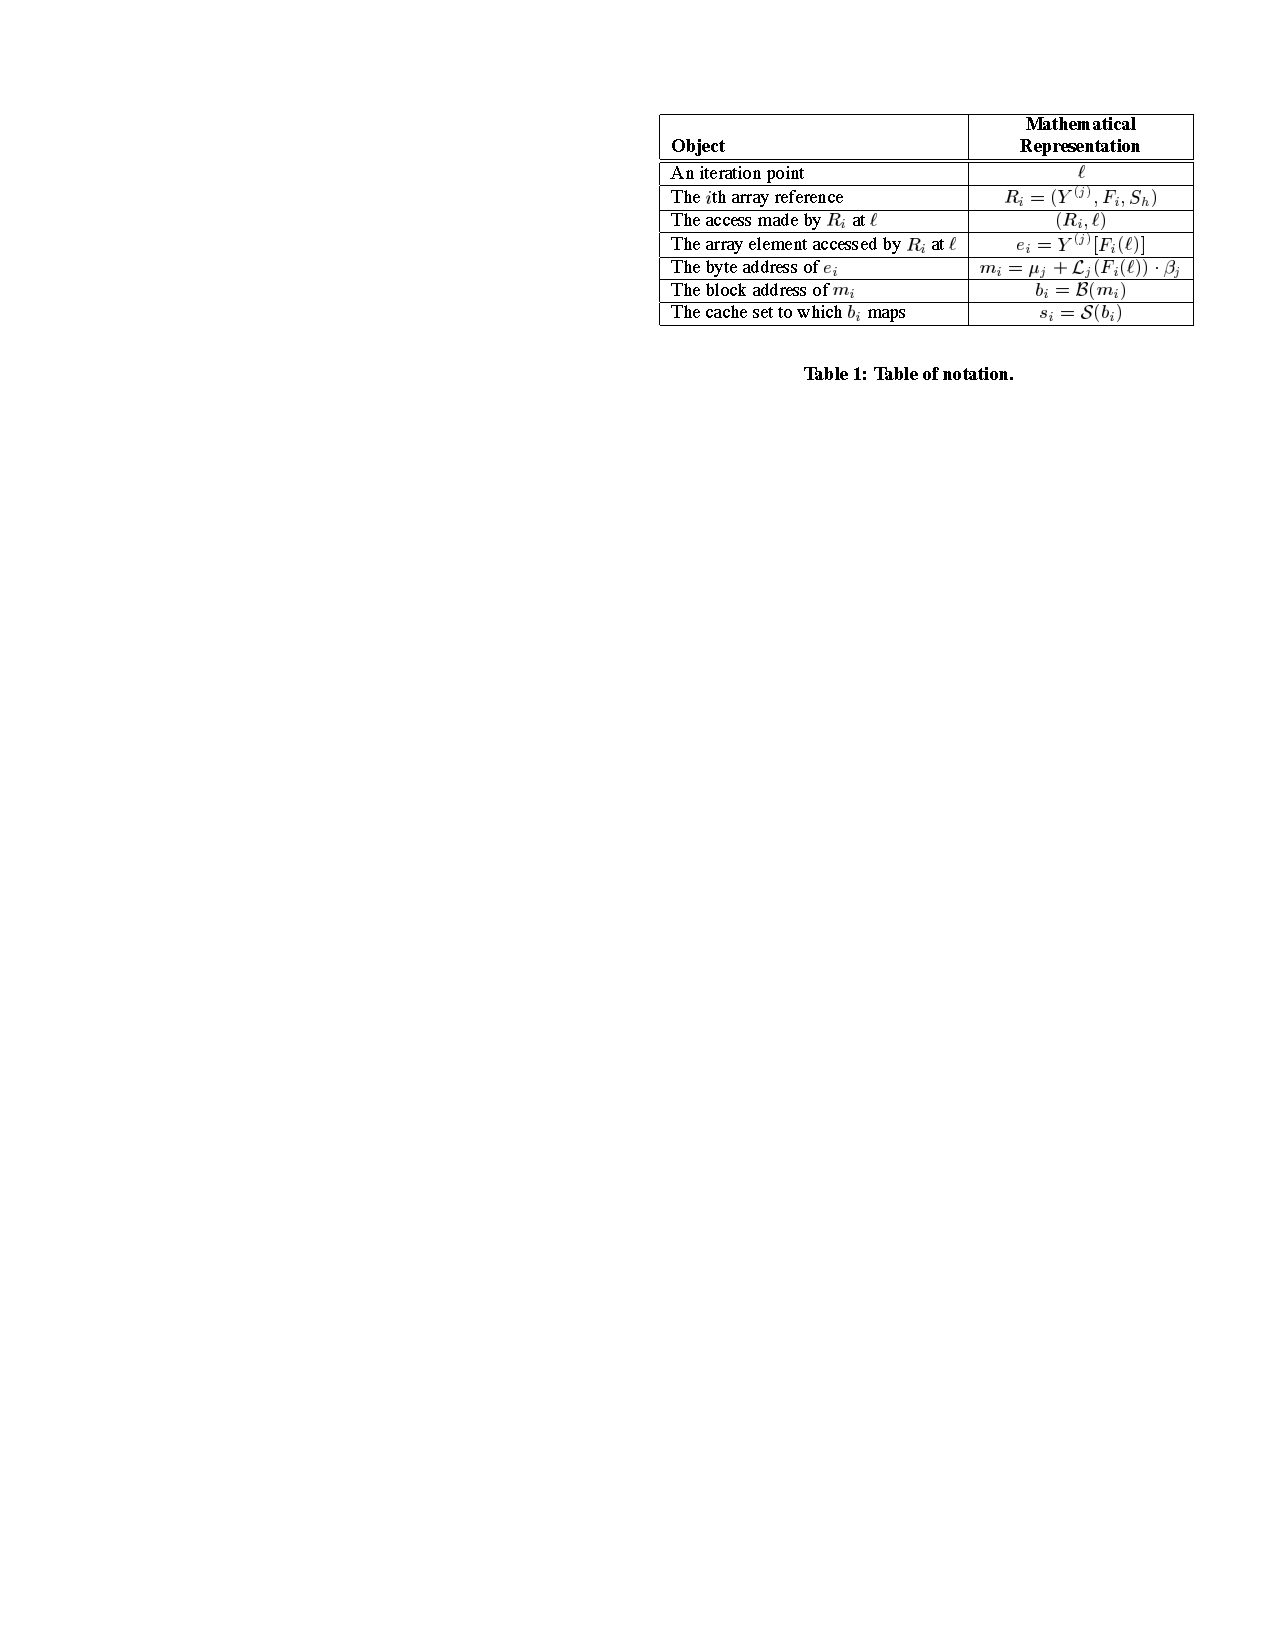
\includegraphics[trim={0 0.6cm 0 0}, clip, scale=1.1]{table1}
  \end{center}

  \begin{itemize}
    \item An iteration point is an array of indexes.
  \end{itemize}
\end{frame}

\begin{frame}{Presburger Arithmetic}
  Subset of first order logic
  \begin{description}
    \item[Constraints] Equalities or inequalities
    \item[Operators] $\neg$, $\wedge$ and $\vee$
    \item[Quantifiers] $\forall$ and $\exists$
  \end{description}
  \vfill
  Used to describe cache structure and accesses
\end{frame}


\section{Cache Analysis Model}

\begin{frame}{Valid Iteration Point}
  Express that every index is in the boundaries of its loop.
  \begin{center}
    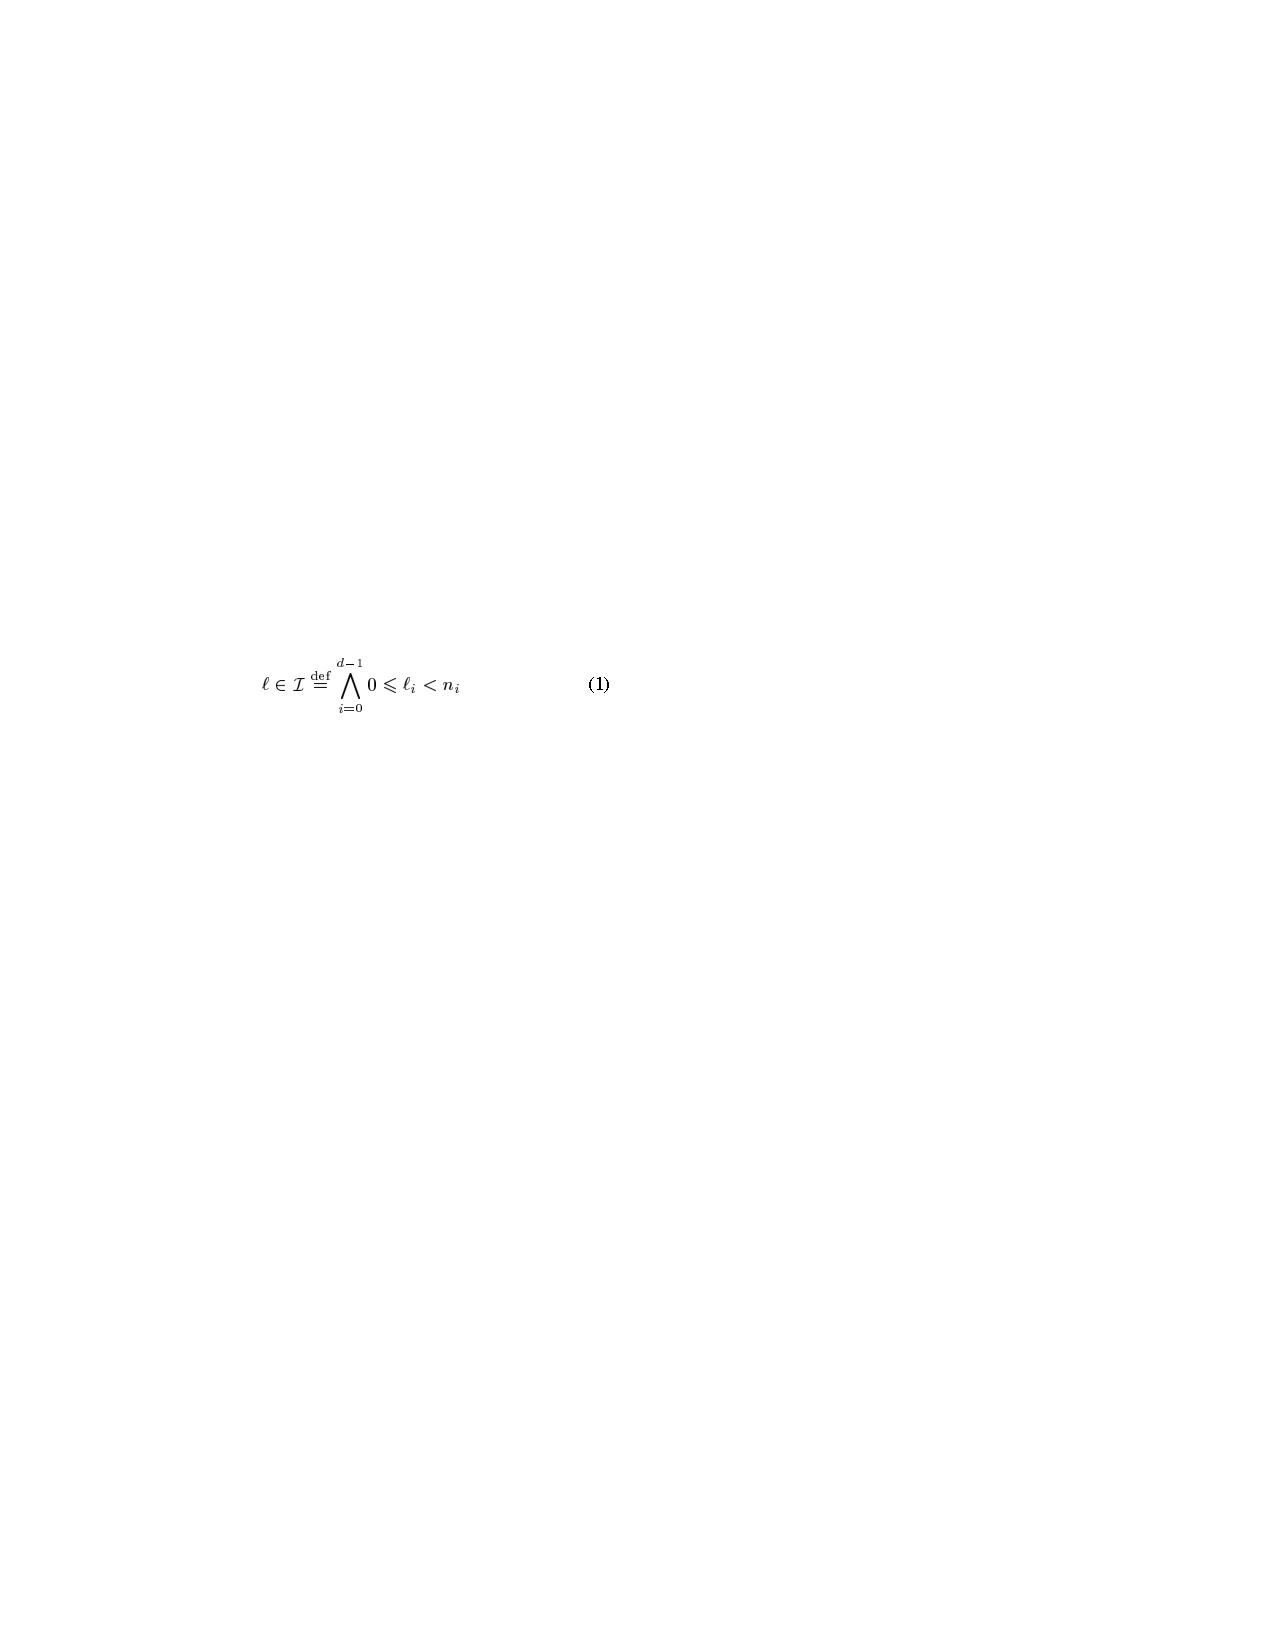
\includegraphics[scale=1.1]{eq1}
  \end{center}
\end{frame}

\begin{frame}{Ordering of Accesses}
  Having an access being done before another means that:
  \begin{itemize}[<+->]
    \item the iteration point is preceding;
    \item or the reference is preceding.
  \end{itemize}
  \begin{center}
    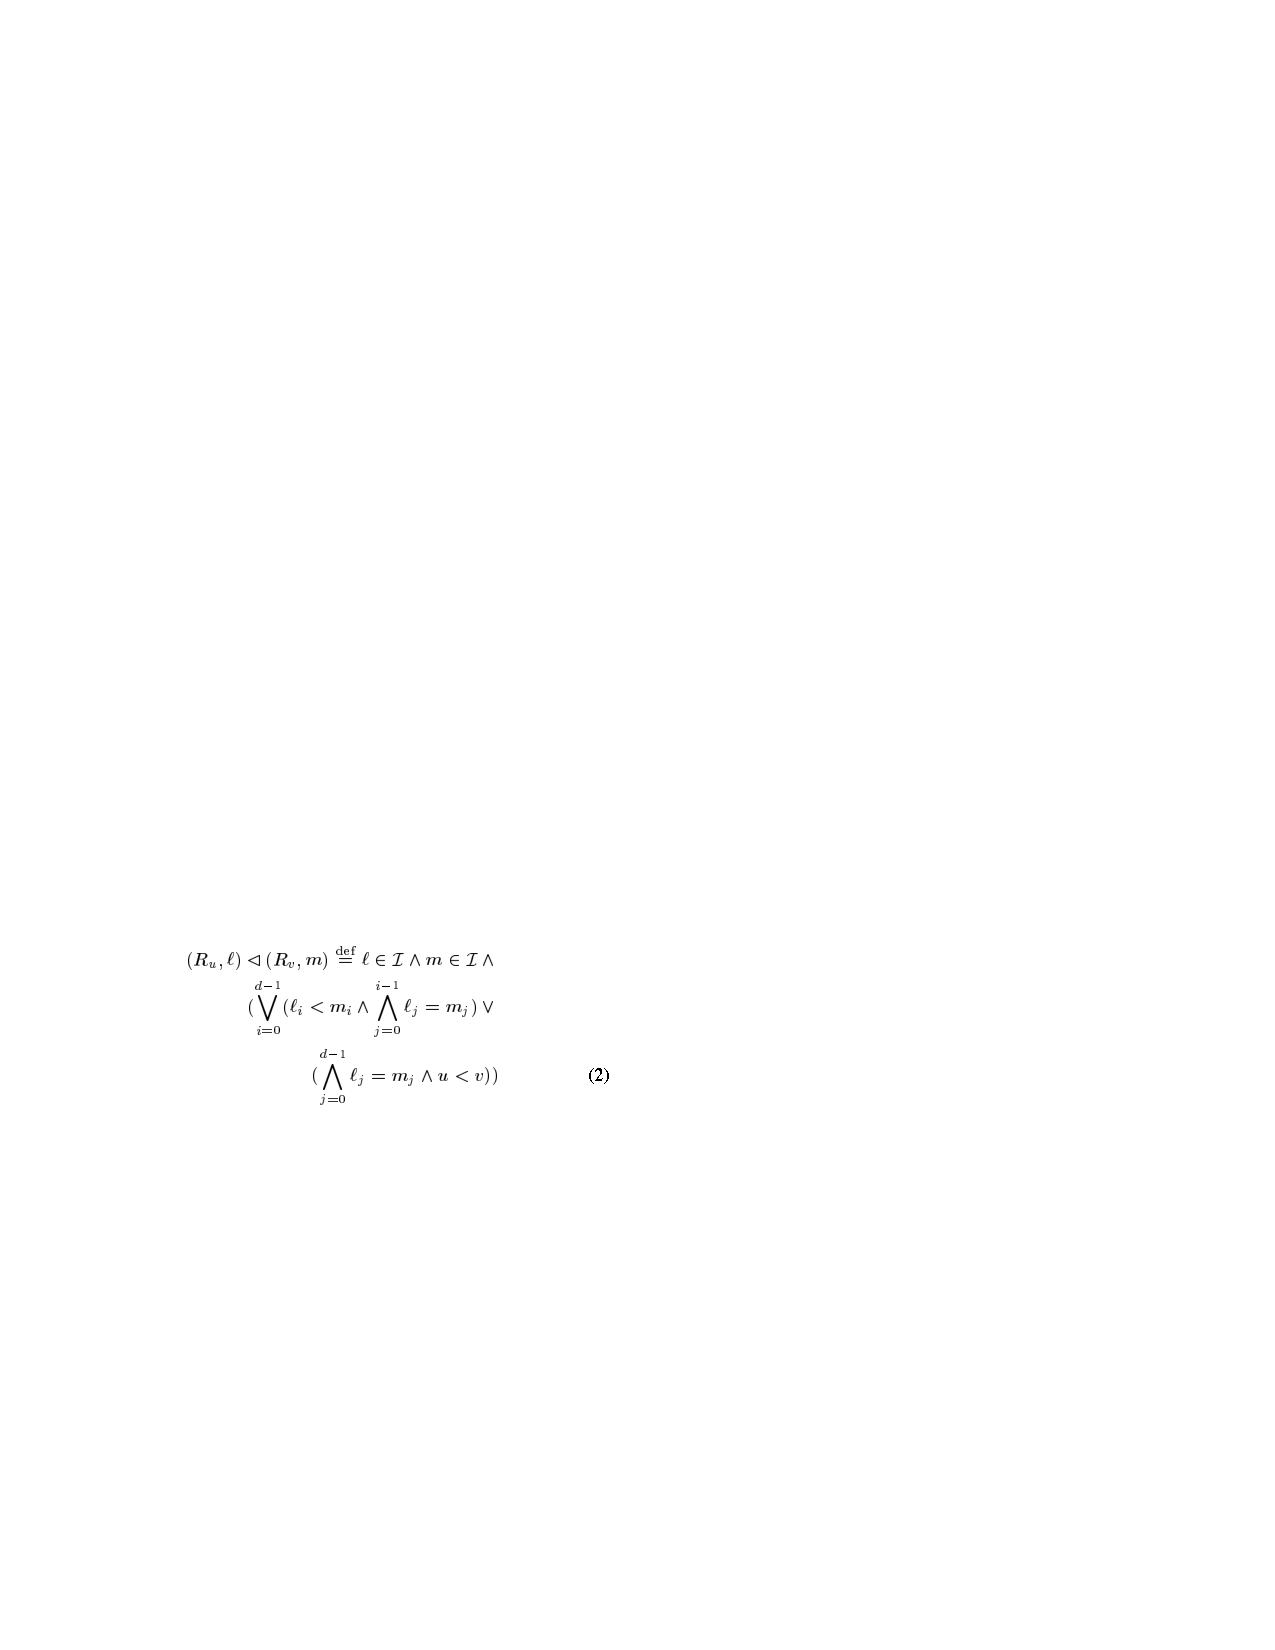
\includegraphics[scale=1.1]{eq2}
  \end{center}
\end{frame}

\begin{frame}{Memory-Cache Mapping}
  Direct mapping.
  \begin{itemize}
    \item Express boundaries of memory address with cache set's boundaries addresses.
    \item Take into account memory block boundary alignments.
  \end{itemize}
  % \begin{center}
  %   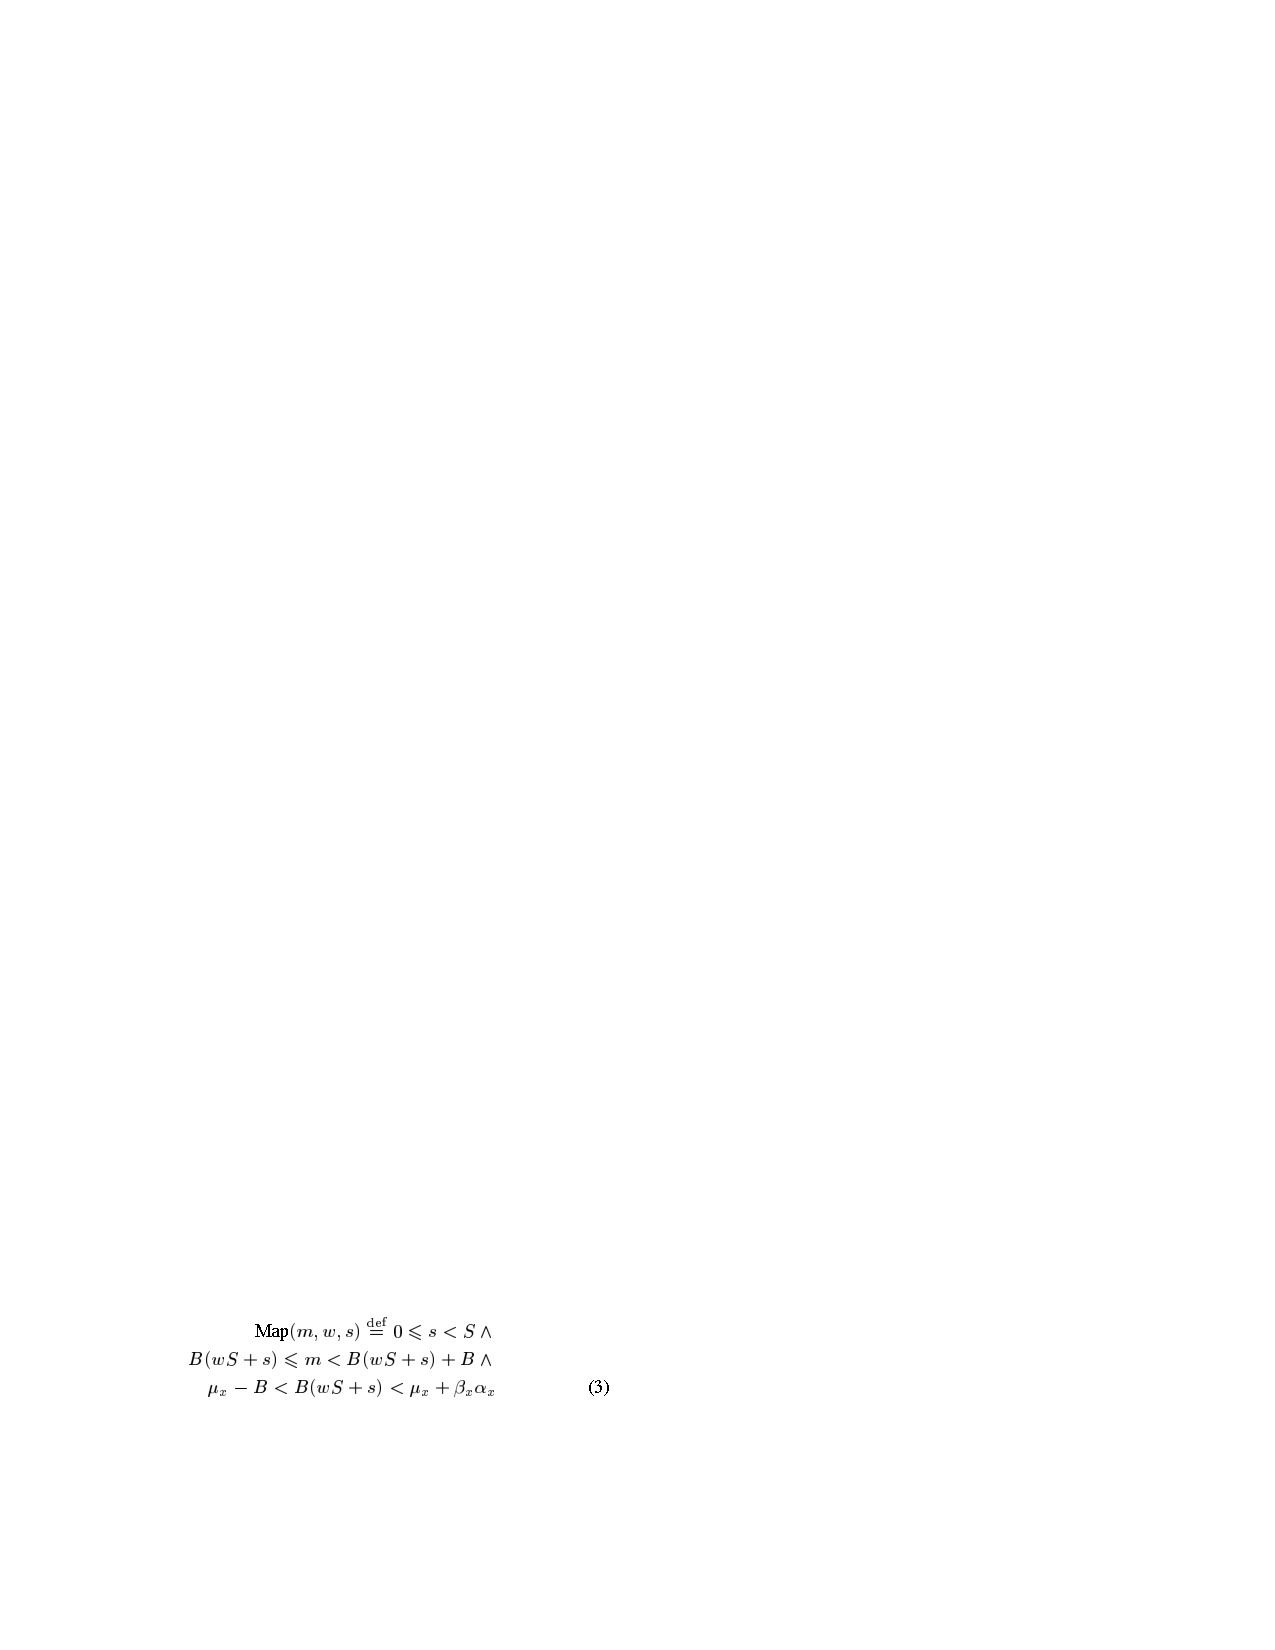
\includegraphics[scale=1.1]{eq3}
  % \end{center}
\end{frame}

\begin{frame}{Boundary Misses}
  Initial state dependent misses.
  \begin{itemize}[<+->]
    \item There is an access for a certain cache set $s$;
    \item it is the first;
    \item the cache set does not correspond to the correct memory block.
  \end{itemize}
  \begin{center}
    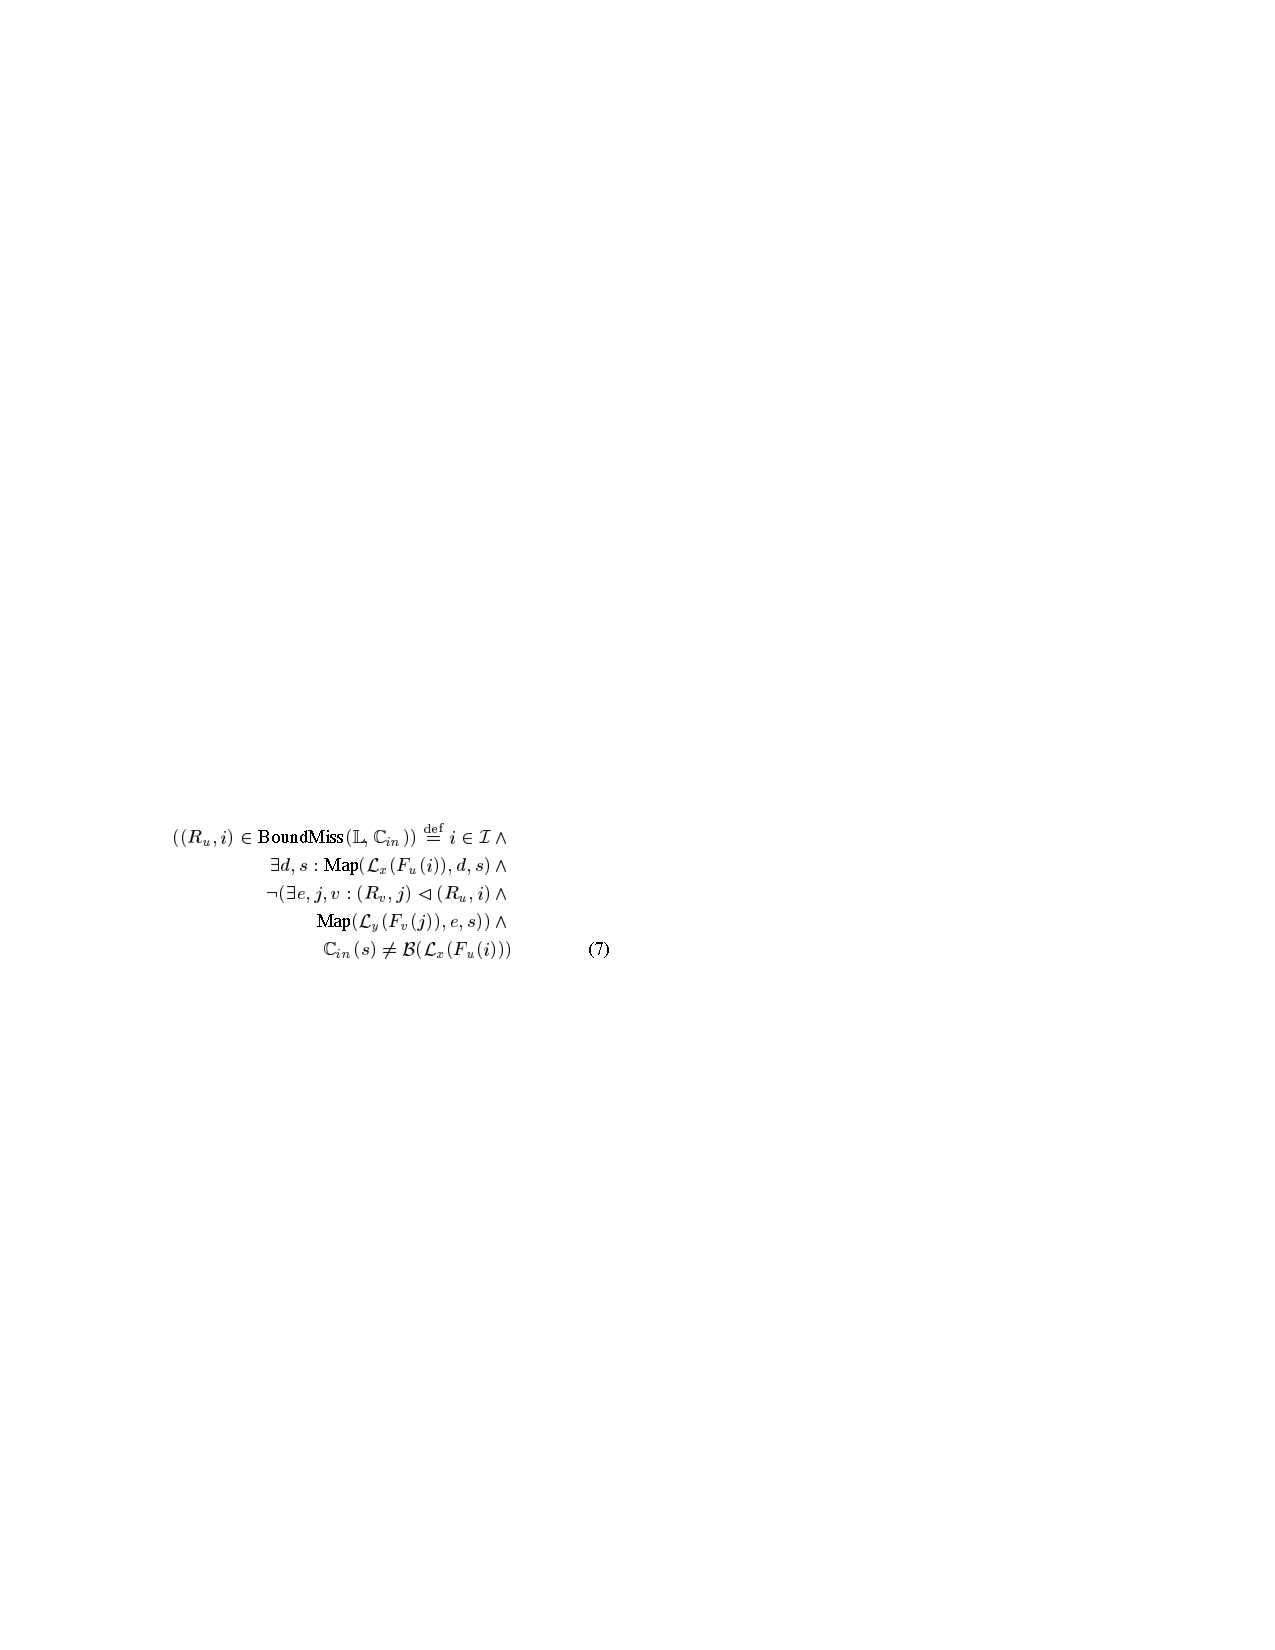
\includegraphics[scale=1.1]{eq7}
  \end{center}
  $\mathcal{L}$ is a layout function (offset of an array element).
  $\mathcal{B}$ is the block address function.
\end{frame}

\begin{frame}{Interior Misses}
  Two properties to have an interior miss for memory block $b$:
  \begin{itemize}
    \item there is an earlier access with a different memory block mapping to the same cache set;
    \item there is no access to $b$ between the two access.
  \end{itemize}
\end{frame}


\section{Extensions}

\begin{frame}{Imperfect Loop Nests}
  Transformation~\cite{ahmed2001synthesizing} with guards on statements.
  \begin{center}
    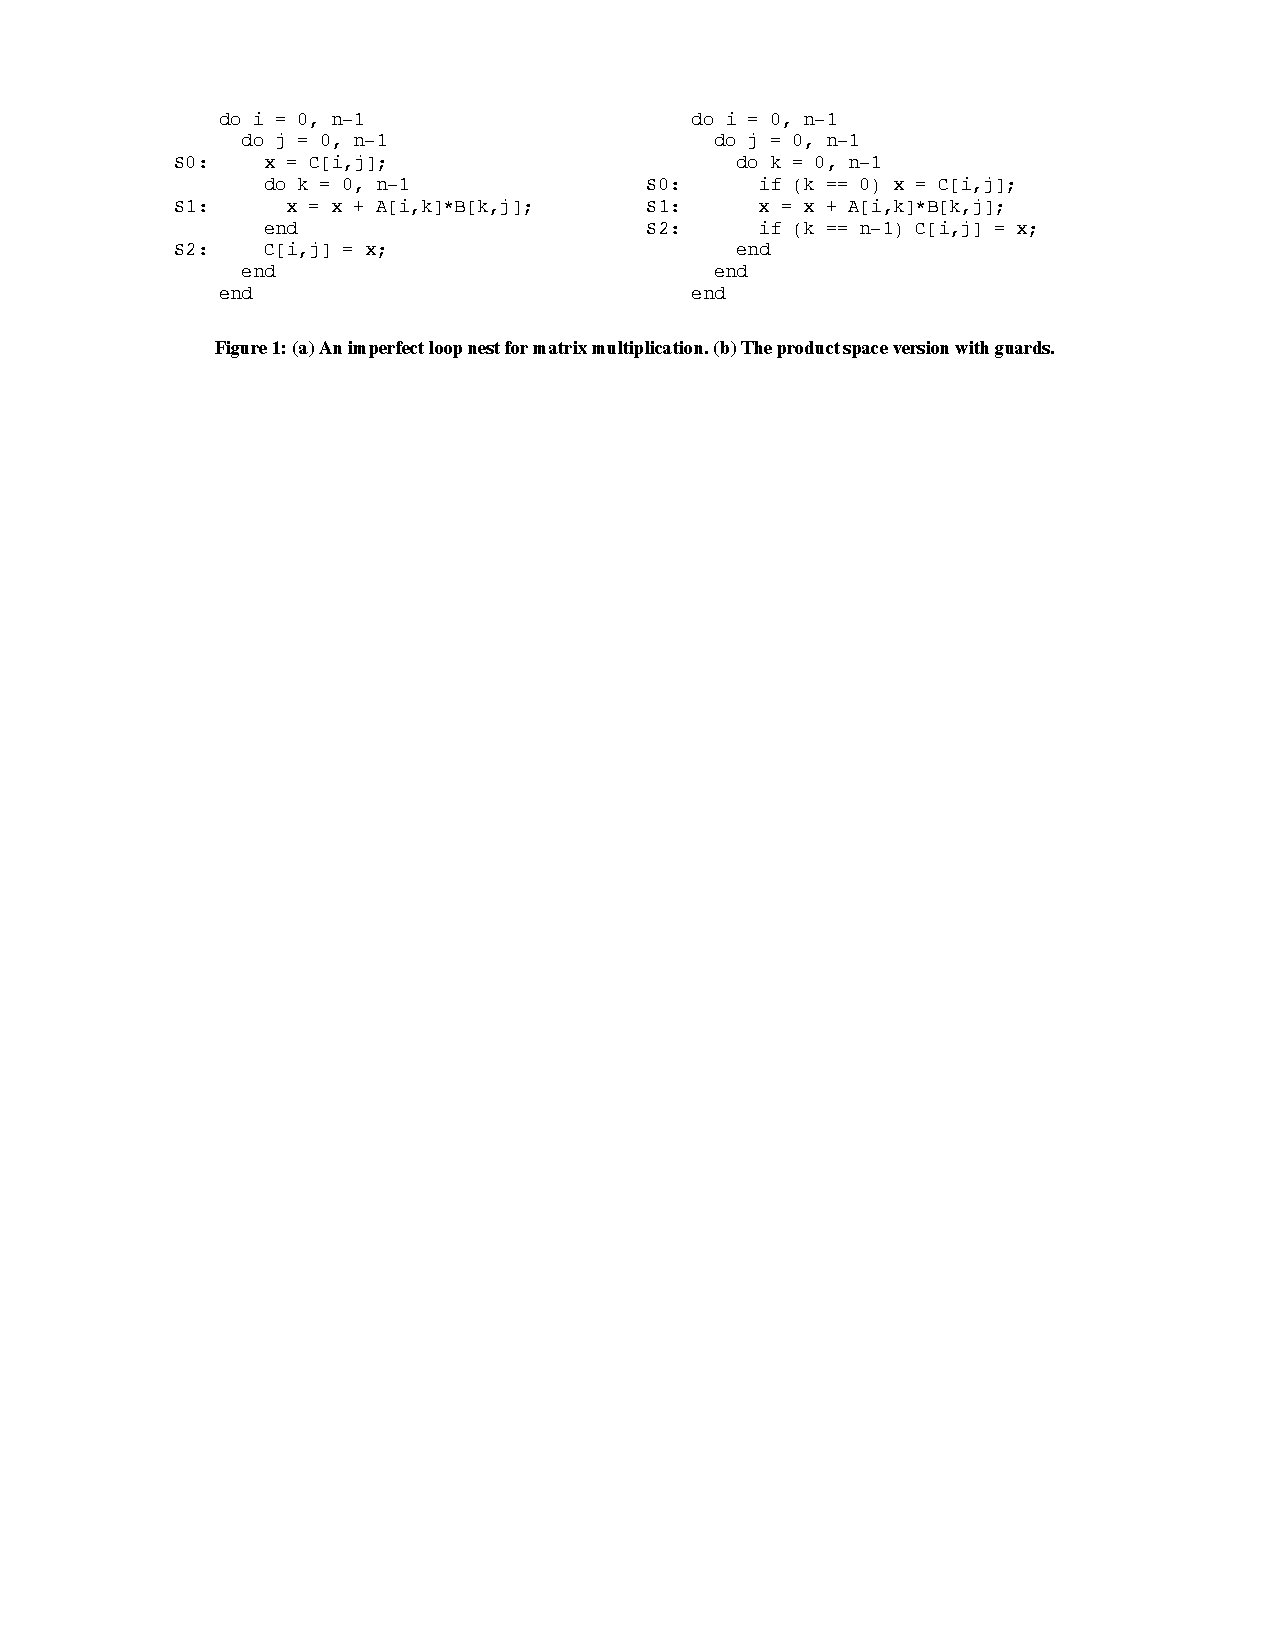
\includegraphics[trim={0 0.6cm 0 0}, clip, width=1.1\textwidth]{figure1}
  \end{center}
  Use \texttt{if}s conditions to express \textit{valid accesses}.
\end{frame}

\begin{frame}{A-way Set-associativity}
  Complicated formula and not efficient.

  \say{Will require more consideration.}

  \begin{center}
    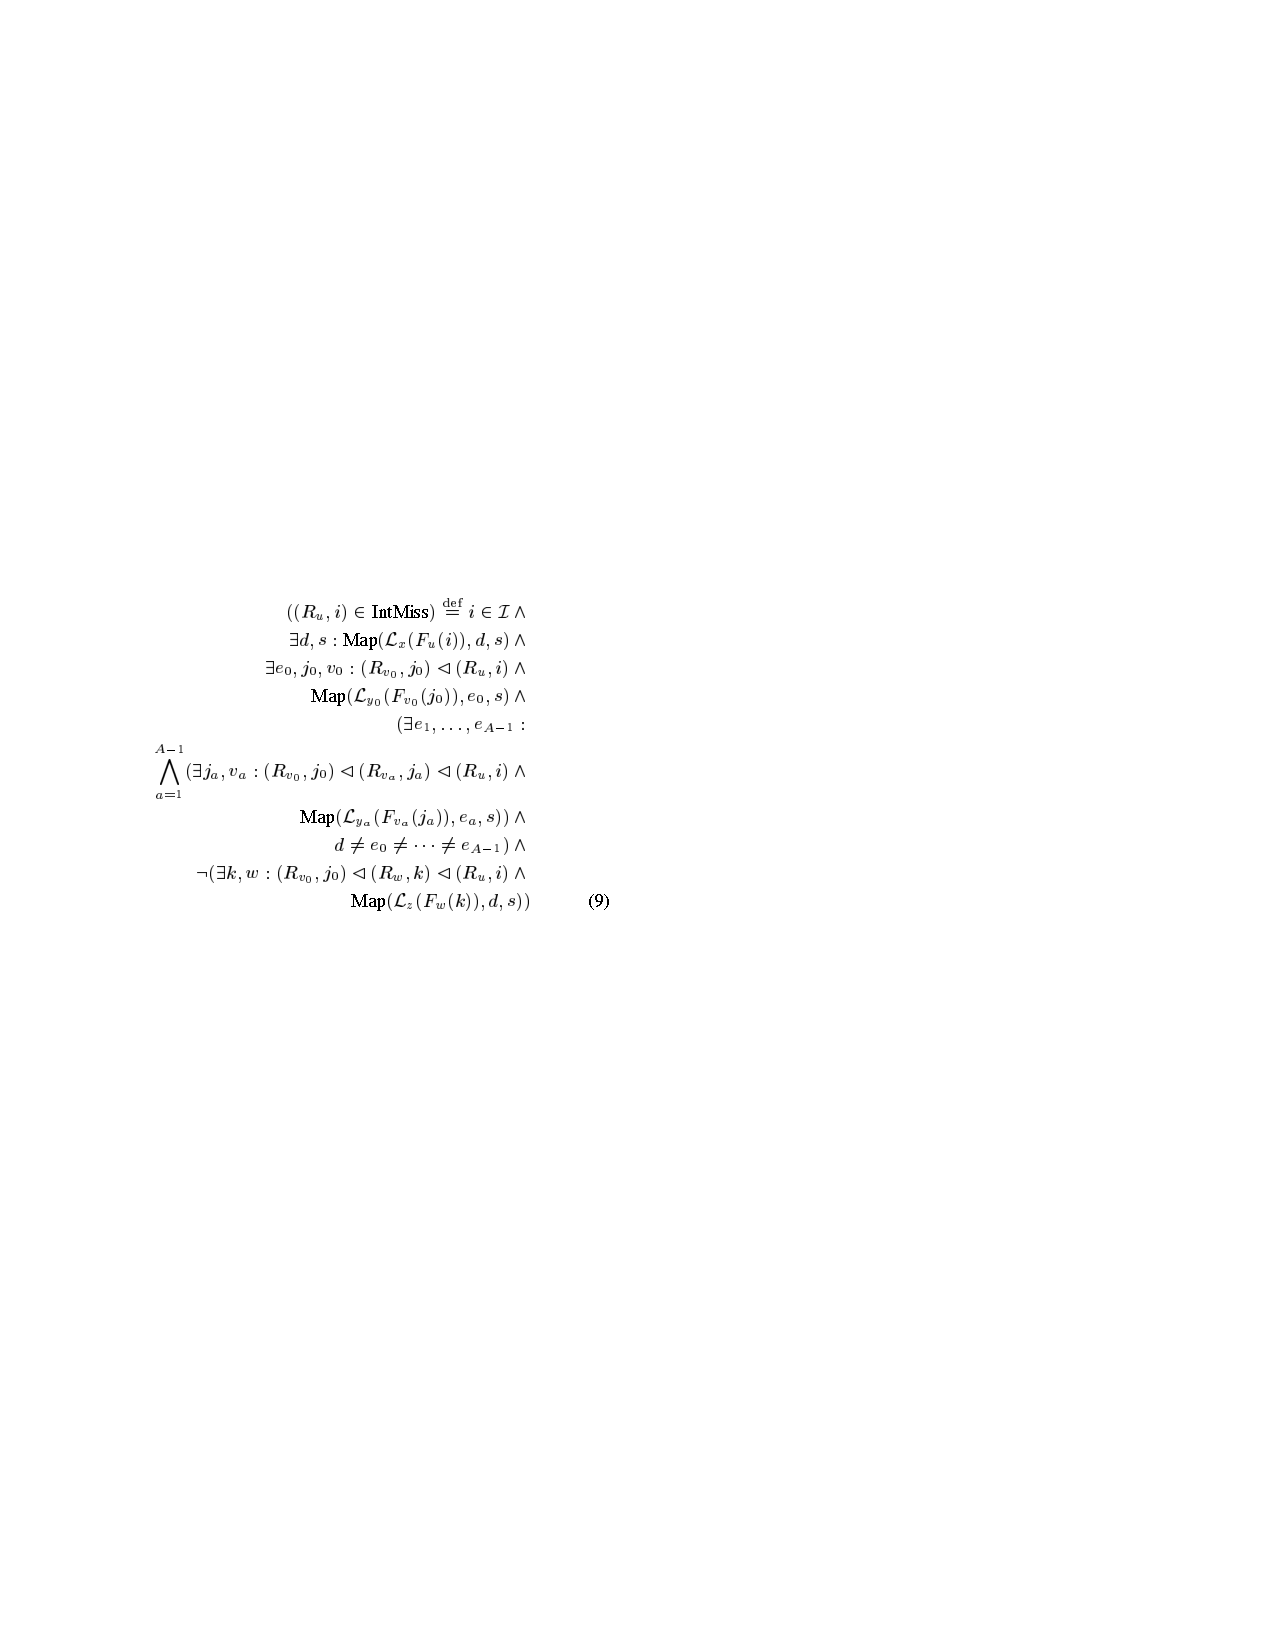
\includegraphics[scale=1.1]{eq9}
  \end{center}
\end{frame}

\begin{frame}{Non-linear Data Layouts}
  Express the data layout's binary manipulations in a Presburger formula.
\end{frame}


\section{Evaluation}

\begin{frame}{Evaluation Method}
  \begin{itemize}
    \item Experimental evaluation
    \item Comparison with cache simulation
    \item Multiple programs used to evaluate every extension
    \item All loop permutations tested
  \end{itemize}
\end{frame}

\begin{frame}{General Results}
  \begin{figure}
    \begin{mdframed}[backgroundcolor=white]
      \begin{center}
        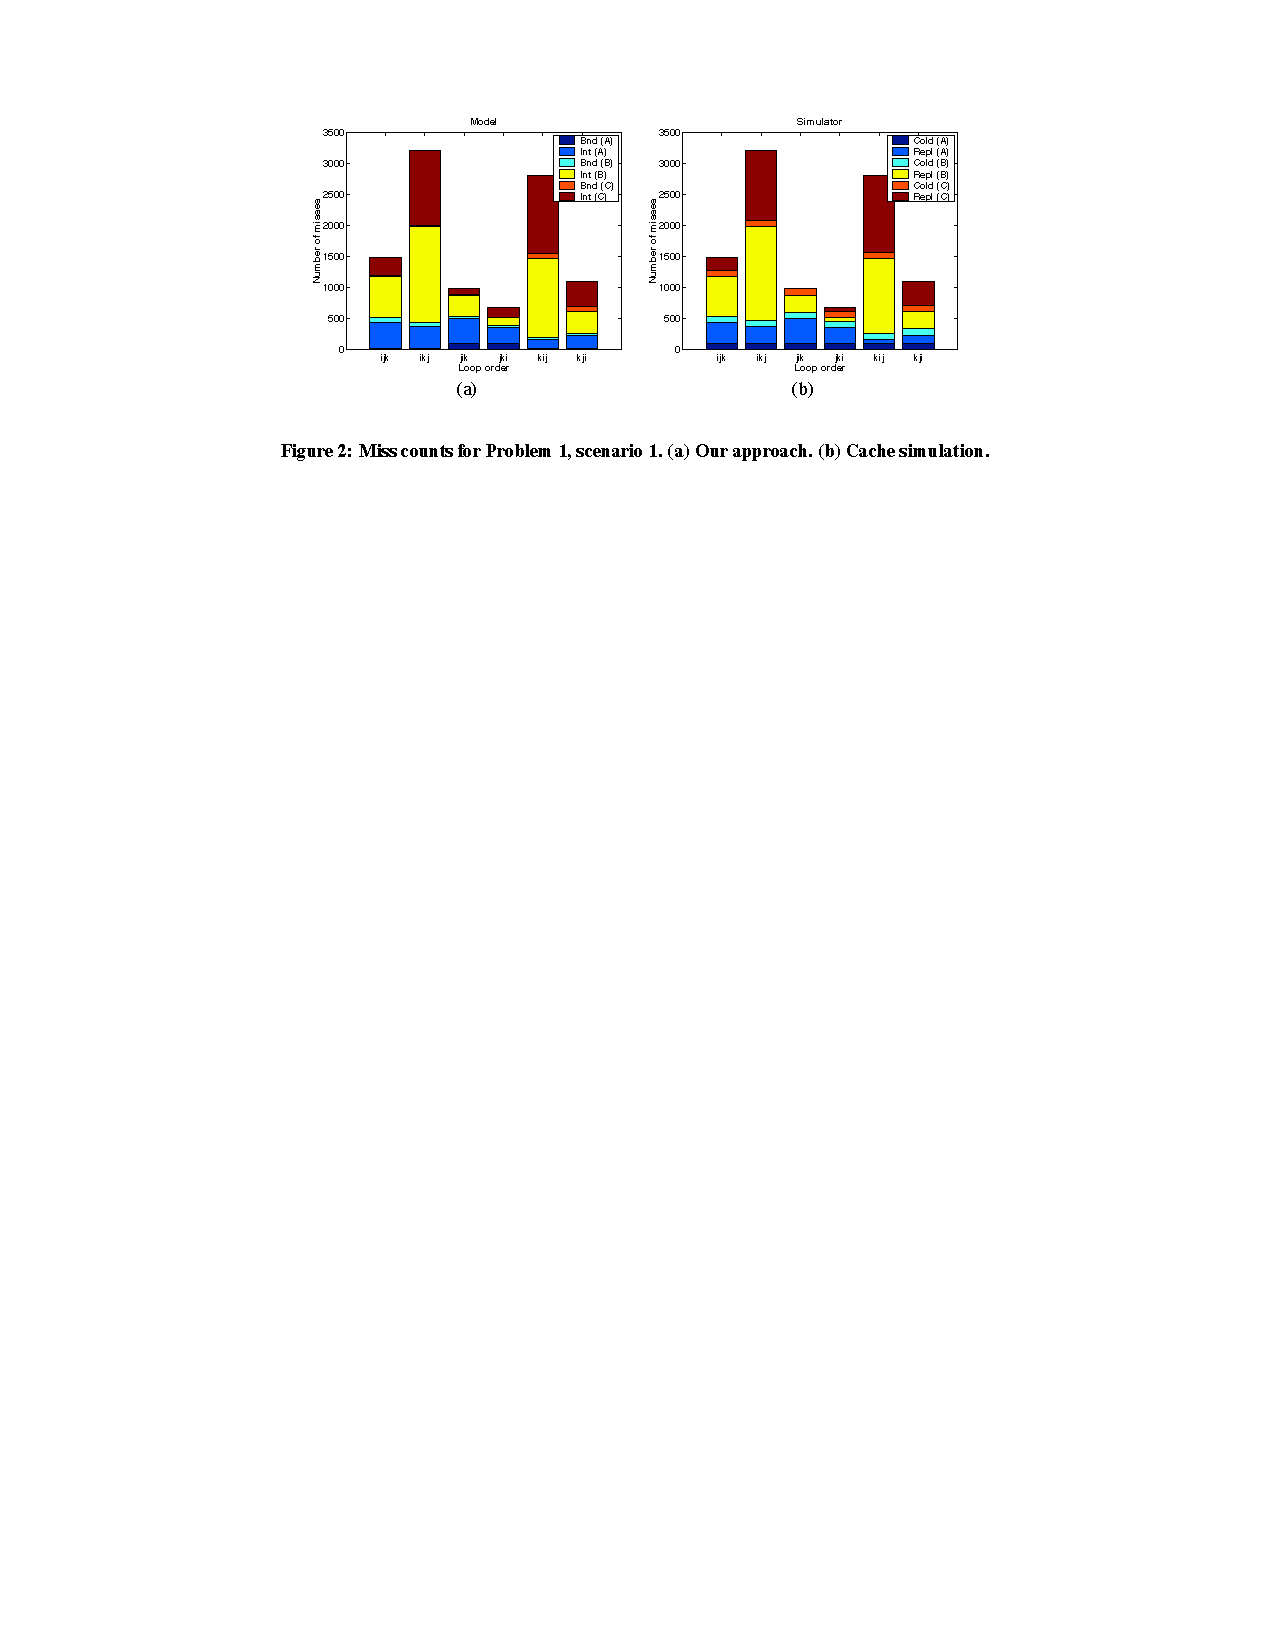
\includegraphics[width=\textwidth]{figure2}
      \end{center}
    \end{mdframed}
  \end{figure}
  \begin{itemize}
    \item Same number of misses
    \item Different classification (\textit{cold} and \textit{replacement} misses)
  \end{itemize}
\end{frame}


\section*{Conclusion}

\begin{frame}{Conclusion}
  \begin{itemize}
    \item Mathematical description for more flexibility in computations
    \item Exploits the regularities of loop nests
    \item Future work: mix simulation and model-based computation to leap-frog loop nests
  \end{itemize}
\end{frame}

\begin{frame}{Critical View}
  \begin{itemize}[<+->]
    \item Assuming one memory access at a time and no distinction between reads and writes seems reasonable
    \item The evaluation convinced me even if I first expected a more formal approach
    \item Still computationally expensive
    \item I believe other policies than LRU could be implemented but the complexity would explode with an A-way set-associativity
    \item Same problem of complexity with more levels of hierarchy
    \item Sometimes confusing variables names between sections
  \end{itemize}
\end{frame}

\appendix

\begin{frame}[allowframebreaks]{References}
  \bibliography{biblio}
  \bibliographystyle{abbrv}
\end{frame}

\end{document}
